\documentclass[11pt]{article}

\usepackage{graphicx}
\usepackage[sort&compress,square,numbers]{natbib}
\usepackage{setspace}

\usepackage{caption}
\usepackage{subcaption}

\bibliographystyle{unsrtnat}

\usepackage{fullpage}
\usepackage{booktabs}
\usepackage{framed}

\usepackage[most]{tcolorbox}
\usepackage{verbatim}
\usepackage{multicol}
\usepackage{multirow}
\usepackage{float}
\usepackage{hyperref}

\topmargin=-0.2in
\textheight=9.5in

\title{
    CSCE 419/614: Term Project\\
    A Study on Ptolemy: Power and Area Analysis}
\author{Insoo Chung (UIN: 232004620)}

\doublespace

\begin{document}
\maketitle
\begin{table}[h] \centering
    \begin{tabular}{lcc}
    \toprule
    \textbf{Evaluation} & \textbf{\begin{tabular}[c]{@{}c@{}}MAX.\\ Score\end{tabular}} & \textbf{\begin{tabular}[c]{@{}c@{}}Your\\ Score\end{tabular}} \\ \midrule
    \begin{tabular}[l]{@{}l@{}}\underline{Overall Organization}\\ Title, abstract (problem attempted, outline of your results,\\ improvements), table of contents, introduction (general\\ description of the problem, motivation, related work, and goals),\\ description of the problem and related definitions and\\ background, description of your work, experimental results,\\ conclusions, appendices (your code may be included here),\\ tables, and figures.\end{tabular} & 10 &  10
    \\ \midrule
    In depth description of the problem and its significance. & 10 &  10
    \\ \midrule
    Techniques used and definitions (should be fairly self-sufficient). & 20 &  20
    \\ \midrule
    Description of your work and results. & 40 &  35
    \\ \midrule
    Technical evaluation (soundness of approach and depth) of results. & 60 &  40
    \\ \midrule
    Conclusions, summary of work, and directions for further work. & 15 &  15
    \\ \midrule
    Appendices (if applicable). & 5 &  5
    \\ \midrule
    References. & 10 &  10
    \\ \midrule
    Overall quality of report. & 30 &  30 \\
    \midrule
    \textbf{Total} & \textbf{200} &  \textbf{175} \\
    \bottomrule
    \end{tabular}
\end{table}

\newpage

\begin{abstract}
    More and more real world products are adopting neural network components. These products generally show good performance to many real world use cases. However, inputs to these components may be pertubated to introduce errors - leaving a room for adversarial attacks. Such attacks can manipulate the output of neural networks, which can be used to cause system to incur real world damage. 
    
    Recently, Ptolemy has been introduced to prevent such attacks at the hardware level. It is claimed that Ptolemy show high accuracy in detecting such attacks, while limiting the computational requirement to a negligible level, preventing Ptolemy from slowing down the overall system.

    In this report, we analyze power and area overhead of Ptolmey modules. The aim of our power and area analysis is to assess the claims of Ptolemy's efficiency by \citeauthor{ptolemy} and to assess the power and area overhead of Ptolemy with respect to design choices. Our estimates show that while area overhead of Ptolemy is marginal to DNN accelerators ($\leq5.7\%$), power overhead from dynamic write can be up to 36.6\%. Furthermore, we show that if we restrict the hardware support to \underline{FwAb} and \underline{BwAb} algorithms which still present good detection accuracy, area and dynamic write overhead can be reduced down to 2.2\% and 21.4\%, respectively.

    
\end{abstract}

\newpage
\tableofcontents
\newpage

\section{Introduction\label{sec:intro}}

In the context of neural networks, \textit{adversarial attacks} refer to attacks on deployed machine learning (ML) models with intention to cause failure. The resulting failures from these attacks may have fatal results. For example, for autonomous driving, a successful attack may result in severe injuries or even death. \citet{szegedy2013intriguing} found that adversarial inputs can be devised to resemble a perfectly well-formed inputs while still causing neural networks to fail. Thus, such attacks may occur in the most discrete forms and could be very hard to prevent.

While various countermeasures have been studied \cite{detected,ensembles}, the studied methods require high computation from fully examining the inputs, and cannot be applied to to be deployed for ML applications that require low latency execution (e.g. autonomous driving). However, more recently proposed Ptolemy \cite{ptolemy} has shown much promise in enabling realtime countermeasures to such attacks.The proposed module was able to achieve high detection accuracy while maintaining a very low detection latency - 2\% runtime overhead as compared to the previous methods. Such feat of efficiency was achieved by focusing on distinctive paths that adversarial inputs activate.

The aim of this term project is to recreate the detector and assess its efficacy. The efficiency of the detector will be measured in terms of area and power overhead of the module implementation. Furthermore, we show that we can make design choices to limit Ptolemy support to \underline{BwAb} and \underline{FwAb} variants to reduce energy and area overhead.

\section{Related Work}

In this section, we will discuss the related work that has been done in the past. In Section \ref{sec:adv}, we discuss training methods that mitigate the effects of adversarial attacks and in Section \ref{sec:countermeasures}, we discuss countermeasures to such attacks. 

\subsection{Adversarial Attack\label{sec:adv}}

\begin{figure}[H]
\begin{center}
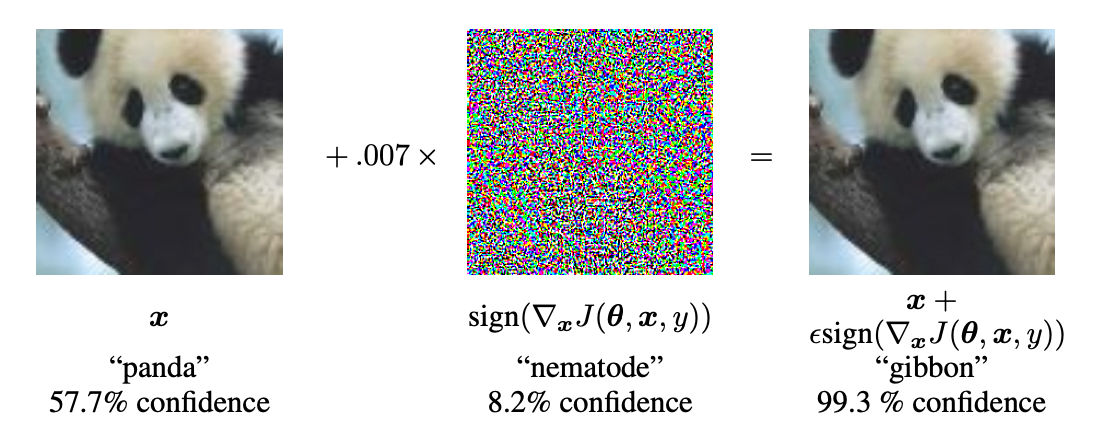
\includegraphics[width=\textwidth]{images/panda.png}
\end{center}
\caption{An adversarial example from \cite{Goodfellow2015adversarial}. Inperceptibily small pertubation can cause neural network classifiers to fail.}
\label{fig:panda}
\end{figure}

\citet{szegedy2013intriguing} found that inputs can be pertubated to cause the neural network to fail without any visual artifact that can be discerned by the human eye. They point out that the smoothness assumption (i.e. that the optimized neural network is a smooth function) does not hold true in many trained models and show that a pertubation function may be utilized to exploit the weakspots of a neural network. Further study by \citet{Goodfellow2015adversarial} showed found that the linearities in of trained models show weakness to adversarial attacks. Also, they showed that simple fast pertubation functions can be used (e.g. Figure \ref{fig:panda}) and that adversarial pertubations are generalizable across different inputs. 

More recent works show that small physical objects can be easily applied to other objects to fool neural networks - which shows adversarial attacks could be done very easily. \citet{2019glasses} show that wearing eyeglasses of a devised design can be used to fool a neural network into perceiving a person as someone else. Also, an adversarial image may be printed out as a sticker patch to be applied to different objects to fool neural network classifiers \cite{brown2018adversarial}. These may not seem to cause any harm, but as more and more AI-based products are deployed and used, depending on the objective of such products, the effect of such attacks can be severe. For example, a couple of small tape strips may be applied to stop signs to cause failure in neural networks in vehicles to fail at detecting when to stop, possibly causing severe harm \cite{stopsign}.

As possibilities of these attacks pose real threat, a several countermeasures have been proposed. In the subsequent subsection, we will discuss the relevant research.



\subsection{Defenses Against Adversarial Attacks\label{sec:countermeasures}}

\paragraph{Adversarial Training}

Adversarial training - in which the model is trained with adversarial inputs - has been suggested to defend against adversarial attacks and has shown successful defense rate in some tasks \cite{buckman2018thermometer, whitebox}. However, the adversarial training methods lead to reduced generalizability and robustness in  the original task \cite{onrecent} or performs suboptimally in the case of a complex original task \cite{buckman2018thermometer}. Furthermore, due to the computational requirements of adversarial training methods, overall training time is increased. Also, to new adversarial attack methods that is unknown at the training time, neural network is vulnerable.

\paragraph{Redundant Architectures}

Other defense methods study utilizing redundancy for robustness against adversarial attacks. \citet{deepfense} introduces multiple \textit{defender modules} to the overall architecture to detect possible exploitation of under-explored input spaces. \citet{imagetransformation} study a defense method that seek robustness from consuming multiple copys of an input with various transformation applied to it. These methods show promising defense rate in the conducted experiments. On the other hand, introduce extra computational overheads are often in multitudes of the original architectures' computations. The overhead of these approaches make them less feasible in real world applications.

\paragraph{Ptolemy}

In our report, we extensively focus on Ptolemy \cite{ptolemy} for several reasons. First, unlike other adversarial training methods, which guides neural network training in different direction, Ptolemy only gathers activation  information and not interfere with the model training itself. This is advantageous over the common adversarial training method because in some cases adversarial training leads models to suboptimal parameter spaces \cite{onrecent}. Also, the implementation of Ptolemy is simple. It involves very little changes to the target neural network accelerator therefore making it an easy addition. Lastly, some of the Ptolemy's variation introduce only negligible overhead to neural network inference. In the following Section \ref{sec:ptolemy}, we discuss the Ptolemy method in more detail. 

\section{Ptolemy\label{sec:ptolemy}}

There are several steps that consist Ptolemy method. Of the steps, we are interested in the physical implementation of Ptolemy and analysis of its area and power consumption. In Section \ref{sec:overview}, we breifly discuss all the steps that consist Ptolemy. And in Section \ref{sec:mac}, we discuss modules of interest in detail before we proceed onto our experimental results.

\subsection{Method Overview\label{sec:overview}}
\begin{figure}[H]
    \begin{center}
    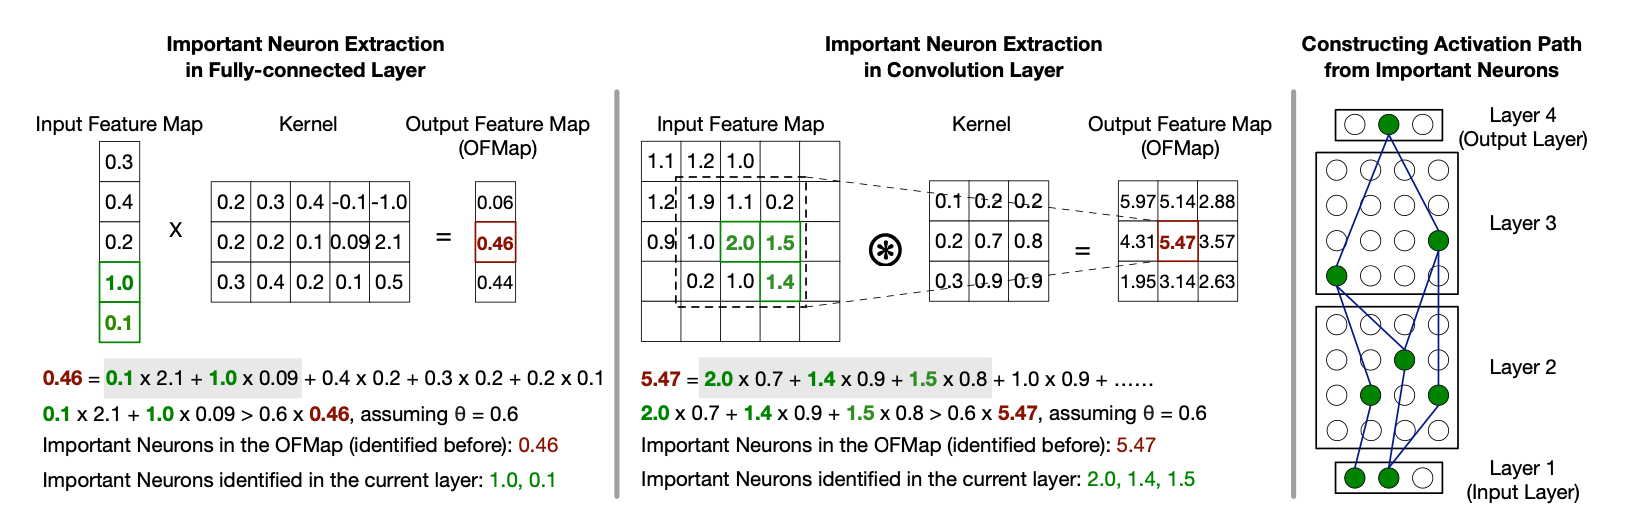
\includegraphics[width=\textwidth]{images/ptolemy.png}
    \end{center}
    \caption{Figure from \cite{ptolemy} showing criterion utilized to select critical neurons during training.}
        \label{fig:criterion}
\end{figure}

The authors utilize the notion of class-level sparsity \cite{identify} to detect adversarial inputs. That is, for a class of output, only a subset of neurons in the whole network is activated. Ptolemy take hints from activation paths \footnote{An activation path is collection of neurons that accumulate to a neural networks final output.} to identify adversarial attacks. For example, if we may observe the \textit{hot path} for an inference run. If the run results in highest probability for an output class \textbf{x}, its \textit{hot path} should resemble the collection of \textit{hot paths} observed during training. Ptolemy authors use this observation to discern adversarial attacks.

Specifically, Ptolemy comprises of offline training phase and online inference phase. \textbf{During the offline training phase}, critical paths for each output class are collected. A path is a set of neurons that contribute highly to the critical neurons in subsequent layers. The path identifying process starts from the output layer, where the only critical neuron is the output class neuron, iterating backward to the input layer. Figure \ref{fig:criterion} show criterion for critical neuron selection. The critical paths are saved as a form of bitmask. All critical paths for an output class is OR-ed into a single critical path mask. \textbf{And in the online inference phase}, the critical path identified for output of each inference run. Then, it is compared against the learned critical path for training for similarity. Simply, authors perform $ mask_{train} \& mask_{run} $ and measure the ratio of $1$s as a similarity metric.

For further details, we refer our readers to the original paper.

\subsection{Runtime Optimization}

Identifying full critical path at the end of neural network execution, pose very high computational overhead when performed in the same way as training - the backward-cumulative (\underline{BwCu}) method. \underline{BwCu} starts its calculation at the end of the inference and require all partial sums during forward propagation to be saved or recalculated. Authors report up to $12.3\times$ latency increase and $7.7\times$ power consumption increase with \underline{BwCu} in AlexNet \cite{alexnet}. With a larger network, ResNet18 \cite{resnet18}, latency and power overhead is $195.4\times$ and $105.9\times$.

To that end, authors suggest optimized variants: forward-absolute (\underline{FwAb}) and backward-absolute (\underline{BwAb}) methods. The \textit{absolute} refers to how critical neurons are identified. Instead of measuring actual contribution of a neuron (Figure \ref{fig:criterion}), the neuron's \textit{absolute} value is compared against a threshold. Identifying the exact set of neurons observing a column of partial sums require a sorting logic and corresponding hardware, which may introduce extensive overhead. Comparing partial sums against an absolute threshold provide a good estimate for our purpose. \citeauthor{ptolemy} reports accuracy $ \approx 90\% $ with AlexNet on ImageNet dataset \cite{imagenet}, which is close to \underline{BwCu}'s $ 95\% $. The high accuracy comes at a low cost, \underline{BwAb} report $1.2\times$ detection latency overhead and $1.1\times$ energy overhead, and \underline{FwAb} report $0.002\times$ detection latency overhead and similar energy overhead. Both methods show substentially low computational requirements as compared to \underline{BwCu}. The \textit{forward} and \textit{backward} portion of the naming refer to the direction of critical path detection. \underline{BwAb} detects critical neurons from output class neuron to start layer. \underline{FwAb} detects critical neurons from start to finish, which enables the method to hide it's latency overhead as path detection can be parallelized with the neural network's inference. However, reported area and energy overhead is similar to \underline{BwAb}. Also, \citeauthor{ptolemy} introduces show further optimizations by examining a subset of all layers can help with computational overheads at a marginal loss of accuracy.

Absolute thresholding provide good accuracy with low computational overhead. Thus, our investigation will be conducted with the scope limited to \underline{FwAb} and \underline{BwAb}.

\begin{figure}[H]
    \begin{center}
    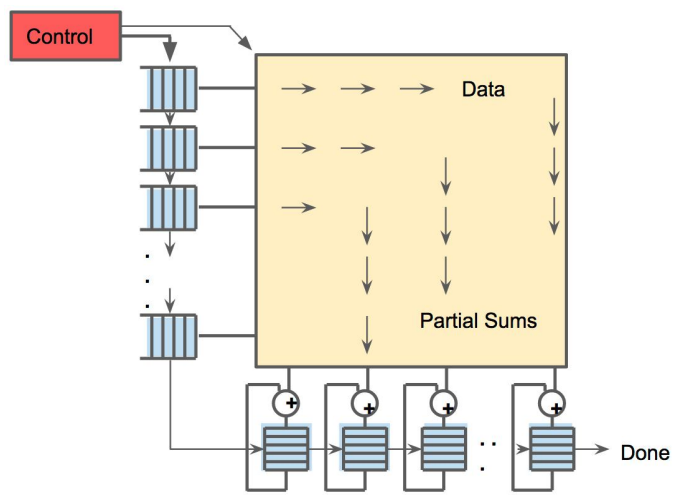
\includegraphics[width=.4\linewidth]{images/systolic-mac.png}
    \end{center}
    \caption{Systolic dataflow of a matrix multipy unit. The illusion of instant matrix multiplication is possible with systolic. Figure from \cite{tpu}. Refer to original paper for elaborate details.}
        \label{fig:tpu}
\end{figure}

\subsection{Hardware Requirements\label{sec:mac}}

\subsubsection{DNN Accelerator}

In their experiments, \citeauthor{ptolemy} assumes of TPU-like design of a systolic array \cite{tpu} incorporating a $20\times20$ MAC array, with each MAC incorporating a two 16-bit fixed-point number inputs to mulitpliers and a 32-bit fixed-point accumulator. The systolic execution flow is illustrated in Figure \ref{fig:tpu}. For this term project, due to time and resource limitations, we do not design a whole DNN accelerator for our experiments. However, as the MAC array is the main compute module of the DNN accelerator, we conjecture that compute overhead analysis limited to the MAC array should provide a good basis for estimating overall DNN accelerator overhead.

\subsubsection{Enhanced MAC Unit}

\begin{figure}[H]
    \centering
    \begin{subfigure}{.45\textwidth}
      \centering
      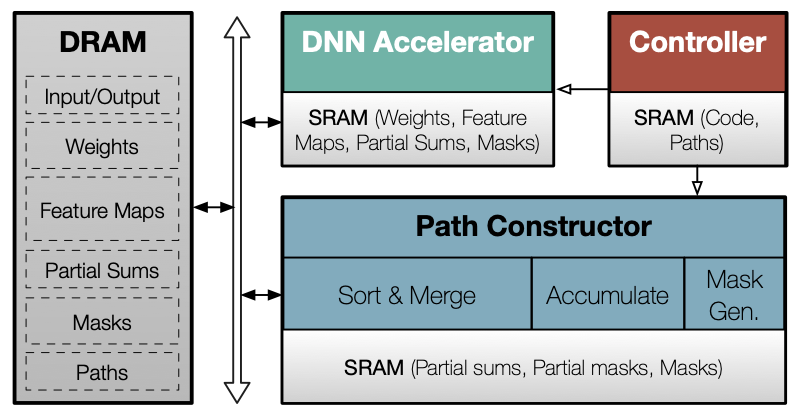
\includegraphics[width=.8\linewidth]{images/hw.png}
    \end{subfigure}
    \begin{subfigure}{.45\textwidth}
      \centering
      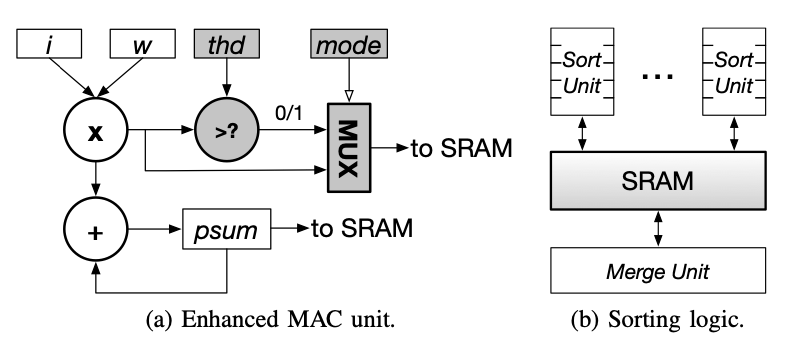
\includegraphics[width=.8\linewidth]{images/aug.png}
    \end{subfigure}
    \caption{Extra hardware required for Ptolemy. Figures are from \cite{ptolemy}. \textbf{(left)} Overall architecture of DNN accelerator with Ptolemy support. \textbf{(right-a)} Augmented MAC unit within DNN accelerator. Gray area is required for \underline{BwAb}, \underline{FwAb}. \textit{psum-to-SRAM} connection is only required for cumulative method, \underline{BwCu}. \textbf{(right-b)} Sorting logic for \underline{BwCu}. \label{fig:mac-aug}}
\end{figure}

Runtime support for adversarial detection requires extra hardware. Figure \ref{fig:mac-aug} show the required hardware for Ptolemy. External to the DNN accelerator, ptolemy require a controller and a path constructor.

Within the DNN accelerator, Ptolemy require extra hardware to perform thresholding (for \underline{BwAb}, \underline{FwAb}). As thresholding is an approximate measure to retreive critical path, \textit{sorting logic is not required}. Sorting logic is only required for methods that extract exact critical path, such as \underline{BwCu}. As our focus is on thresholding methods, we mainly discuss the hardware changes within DNN accelerator: enhanced MAC unit.

\section{Implementations}


\subsection{Softwares}

A set of open-source design tools are utilized for this project. \textbf{icarus-verilog} \cite{icarus} is used to simulate verilog design of MAC modules. \textbf{yosys} \cite{yosys} is used as synthesizer and area estimator of MAC modules. Also, to estmiate power and area of extra SRAM requirements, \textbf{HP-CACTI} \cite{hp-cacti} is used. For versions of utilized tools and verilog implementaion for this project, please refer to the project repository \footnote{\url{https://github.tamu.edu/CSCE-614-Dr-Kim-Fall-21/InsooChung}}. We attempted to utilize a commercial simulator for power and area simulation for MAC design but we failed to yield results within time due to inexperience with all the tools we used/tried-to-use.

\subsection{Design Synthesis}

\subsubsection{Basic Modules}

Simple 32-bit adder that connects a full adder and a half adder in series is used. For multiplicator, a multiplicator implementation that uses booth algorithm and takes two 16-bit fixed-point inputs and outputs a 32-bit fixed-point output is used.

\subsubsection{Matrix Multiplicator Module}

\begin{figure}[H]
    \centering
    \begin{subfigure}{.45\textwidth}
      \centering
      \begin{framed}
        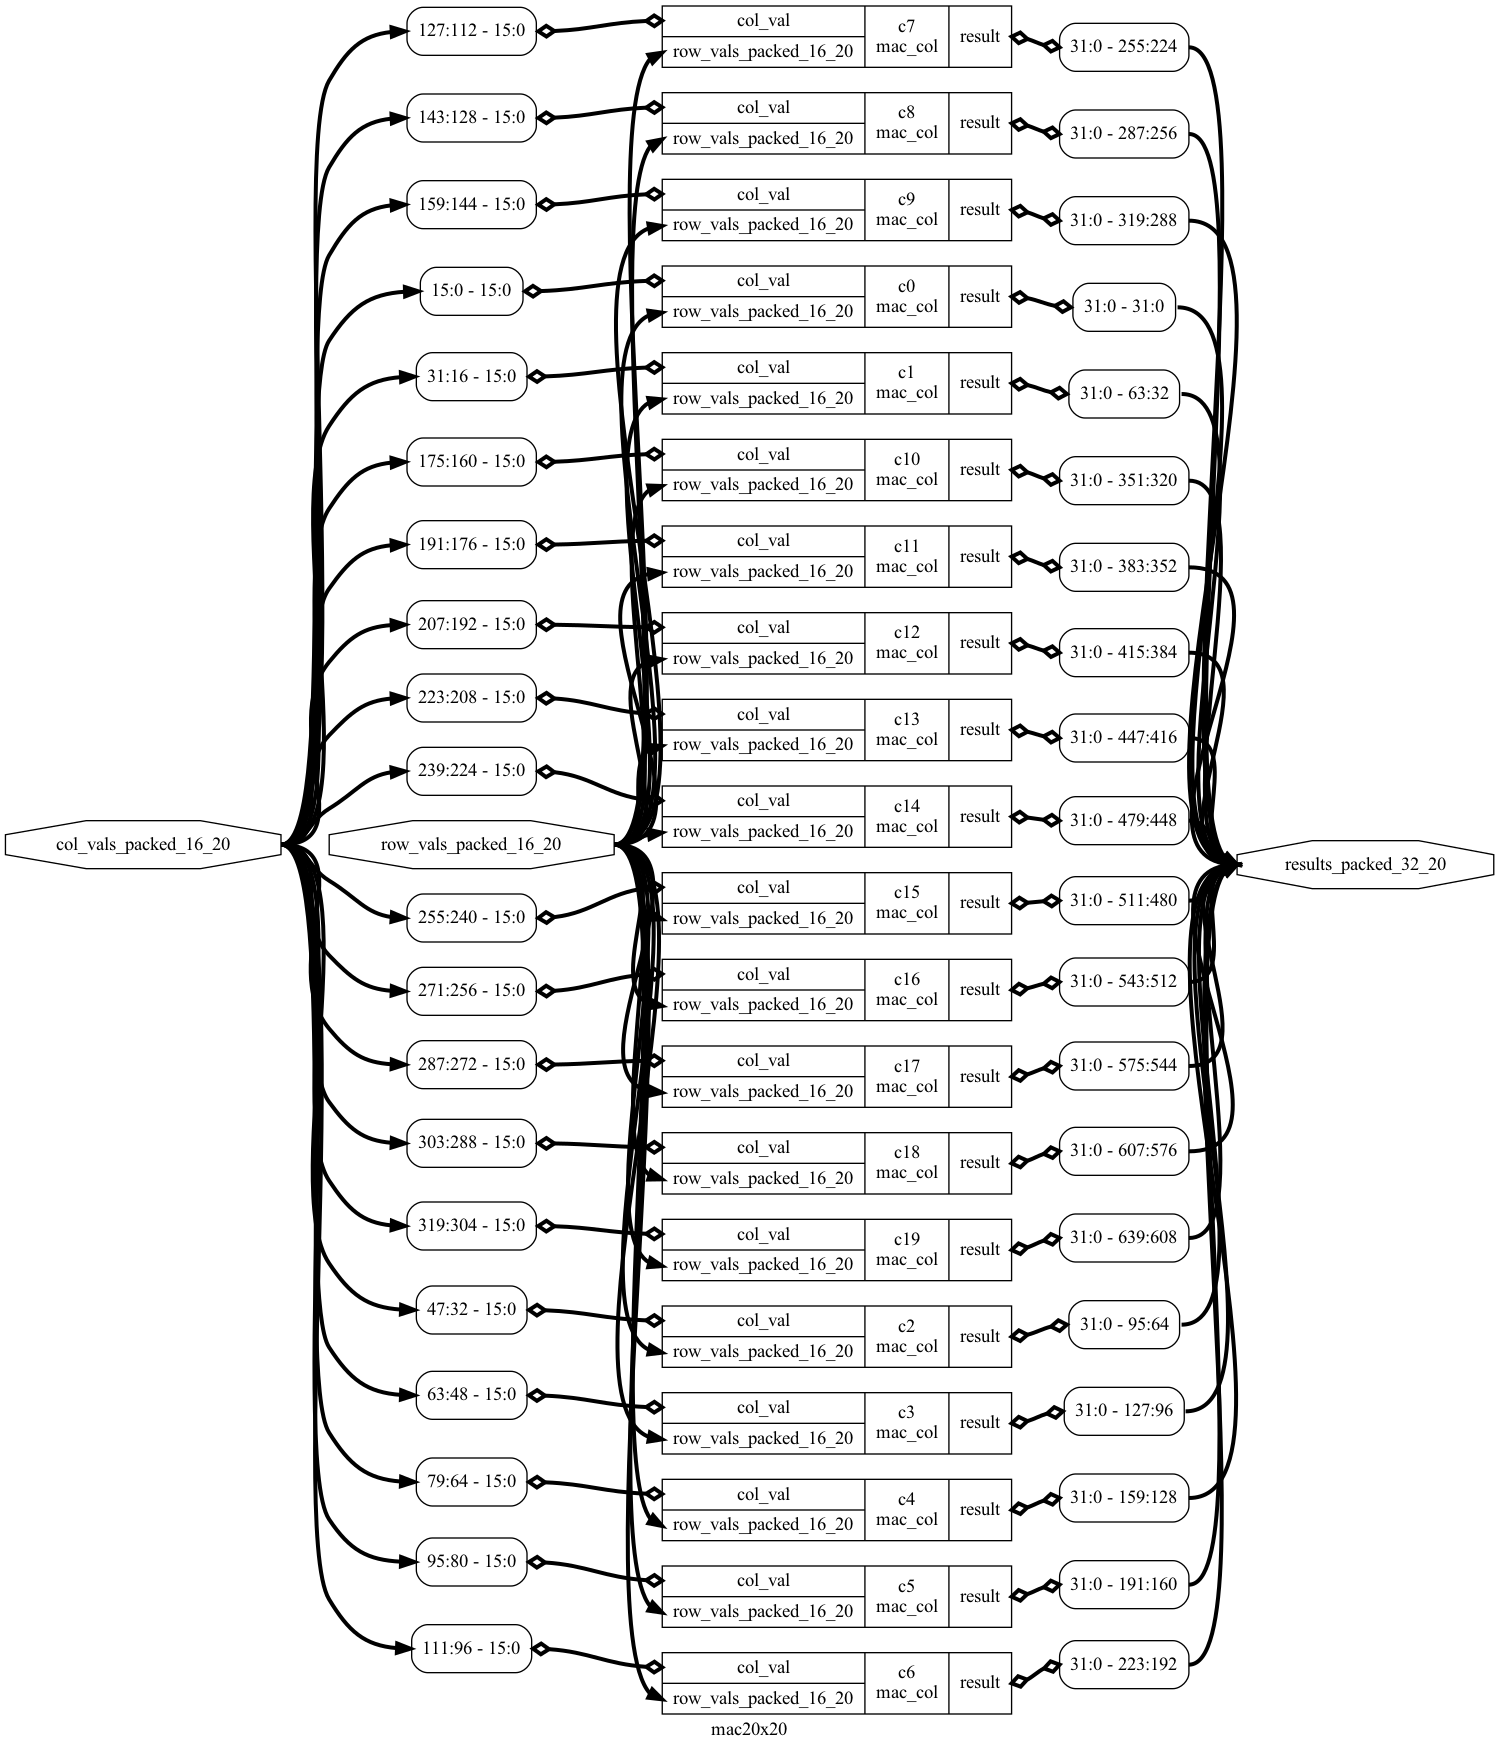
\includegraphics[width=\linewidth]{images/mac20x20.dot.png}
        \caption{20x20 MAC array with systolic dataflow}
      \end{framed}
    \end{subfigure}
    \begin{subfigure}{.45\textwidth}
      \centering
      \begin{framed}
        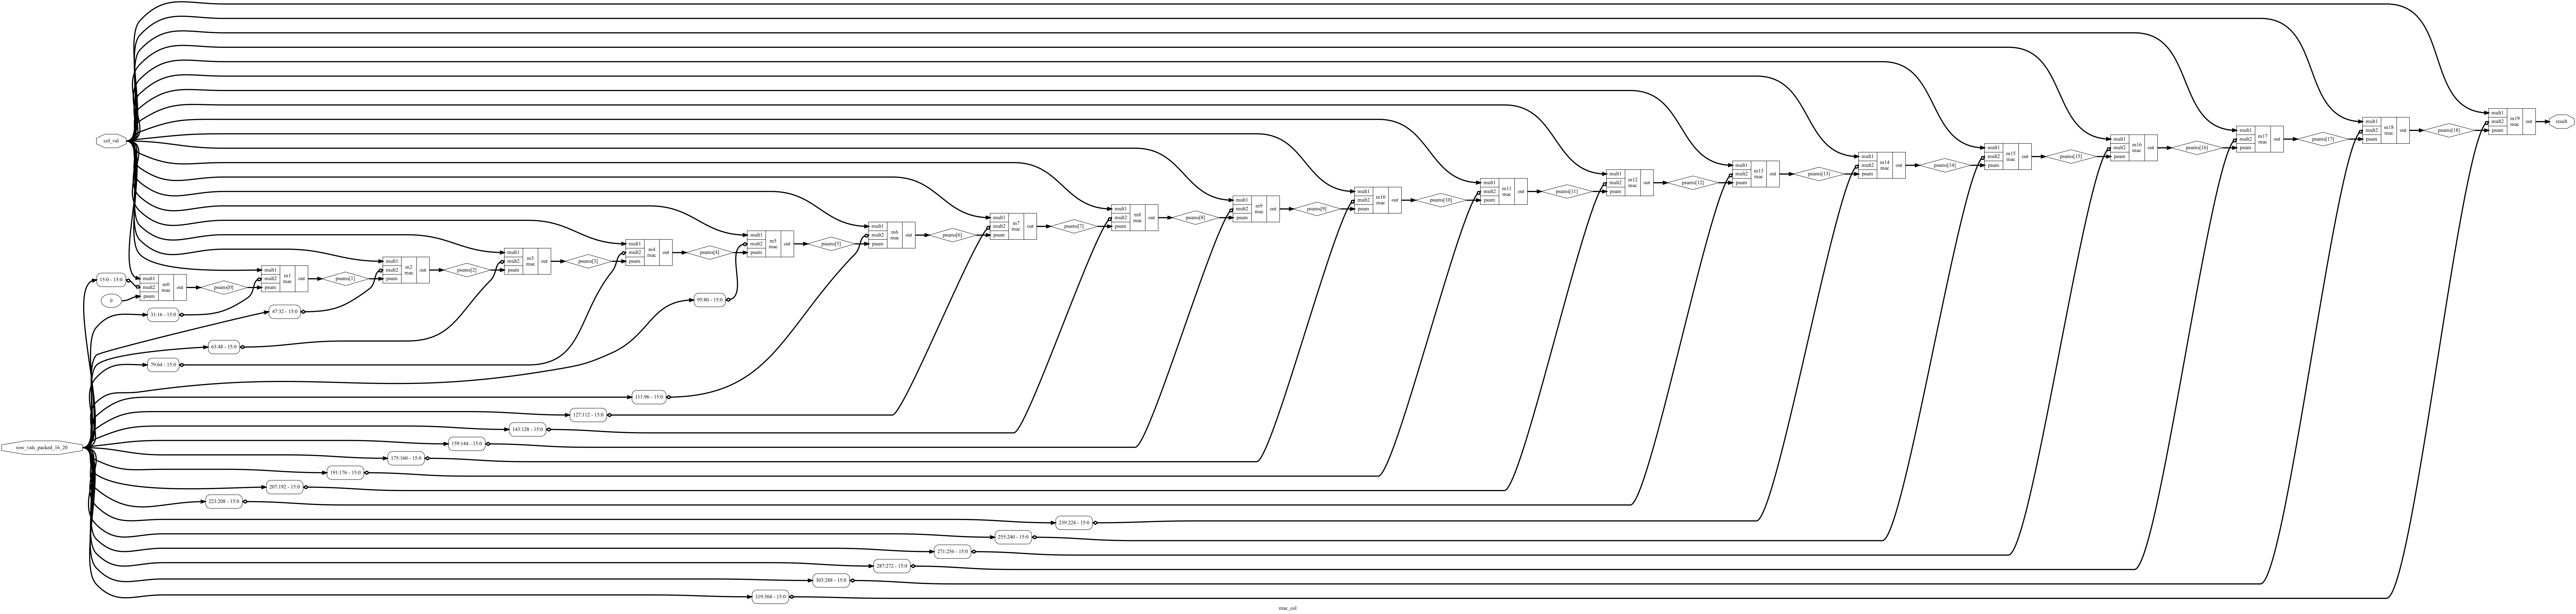
\includegraphics[width=\linewidth]{images/mac_col.dot.png}
        \caption{1x20 MAC column}
      \end{framed}
      \begin{framed}
        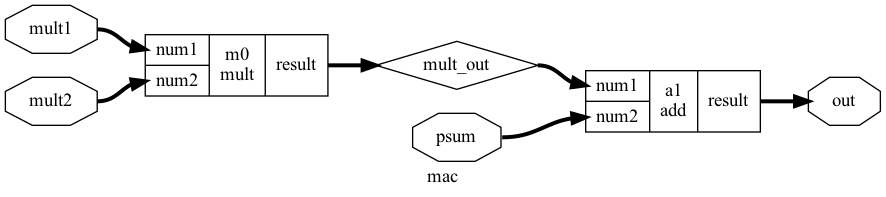
\includegraphics[width=\linewidth]{images/mac.dot.png}
        \caption{Single MAC unit}
      \end{framed}
    \end{subfigure}
    \caption{The 20x20 MAC array that is the main computing unit in vanilla DNN accelerator is illustrated. \textbf{(a)} show its composition in terms of 1x20 MAC columns, \textbf{(b)}. Note that, despite the naming, \textit{column}s are illustrated with a 90-degrees tilt, in a row-like fashion. The design is syntehsized and visualized with \textbf{yosys}.\label{fig:macs}}
\end{figure}

The visualization of implemented the 20x20 MAC array is presented in Figure \ref{fig:macs}. The array follow the TPU-like systolic dataflow. Tests that on the implementation was conducted and the result show 1 clock execution for all multiplication-add operations. Readers may refer to test logs in Appendix \ref{a:mac_test} to examine the implementation's sanity.

\subsubsection{Augmented Matrix Multiplicator Module}

\begin{figure}[H]
    \centering
    \begin{subfigure}{.45\textwidth}
      \centering
      \begin{framed}
        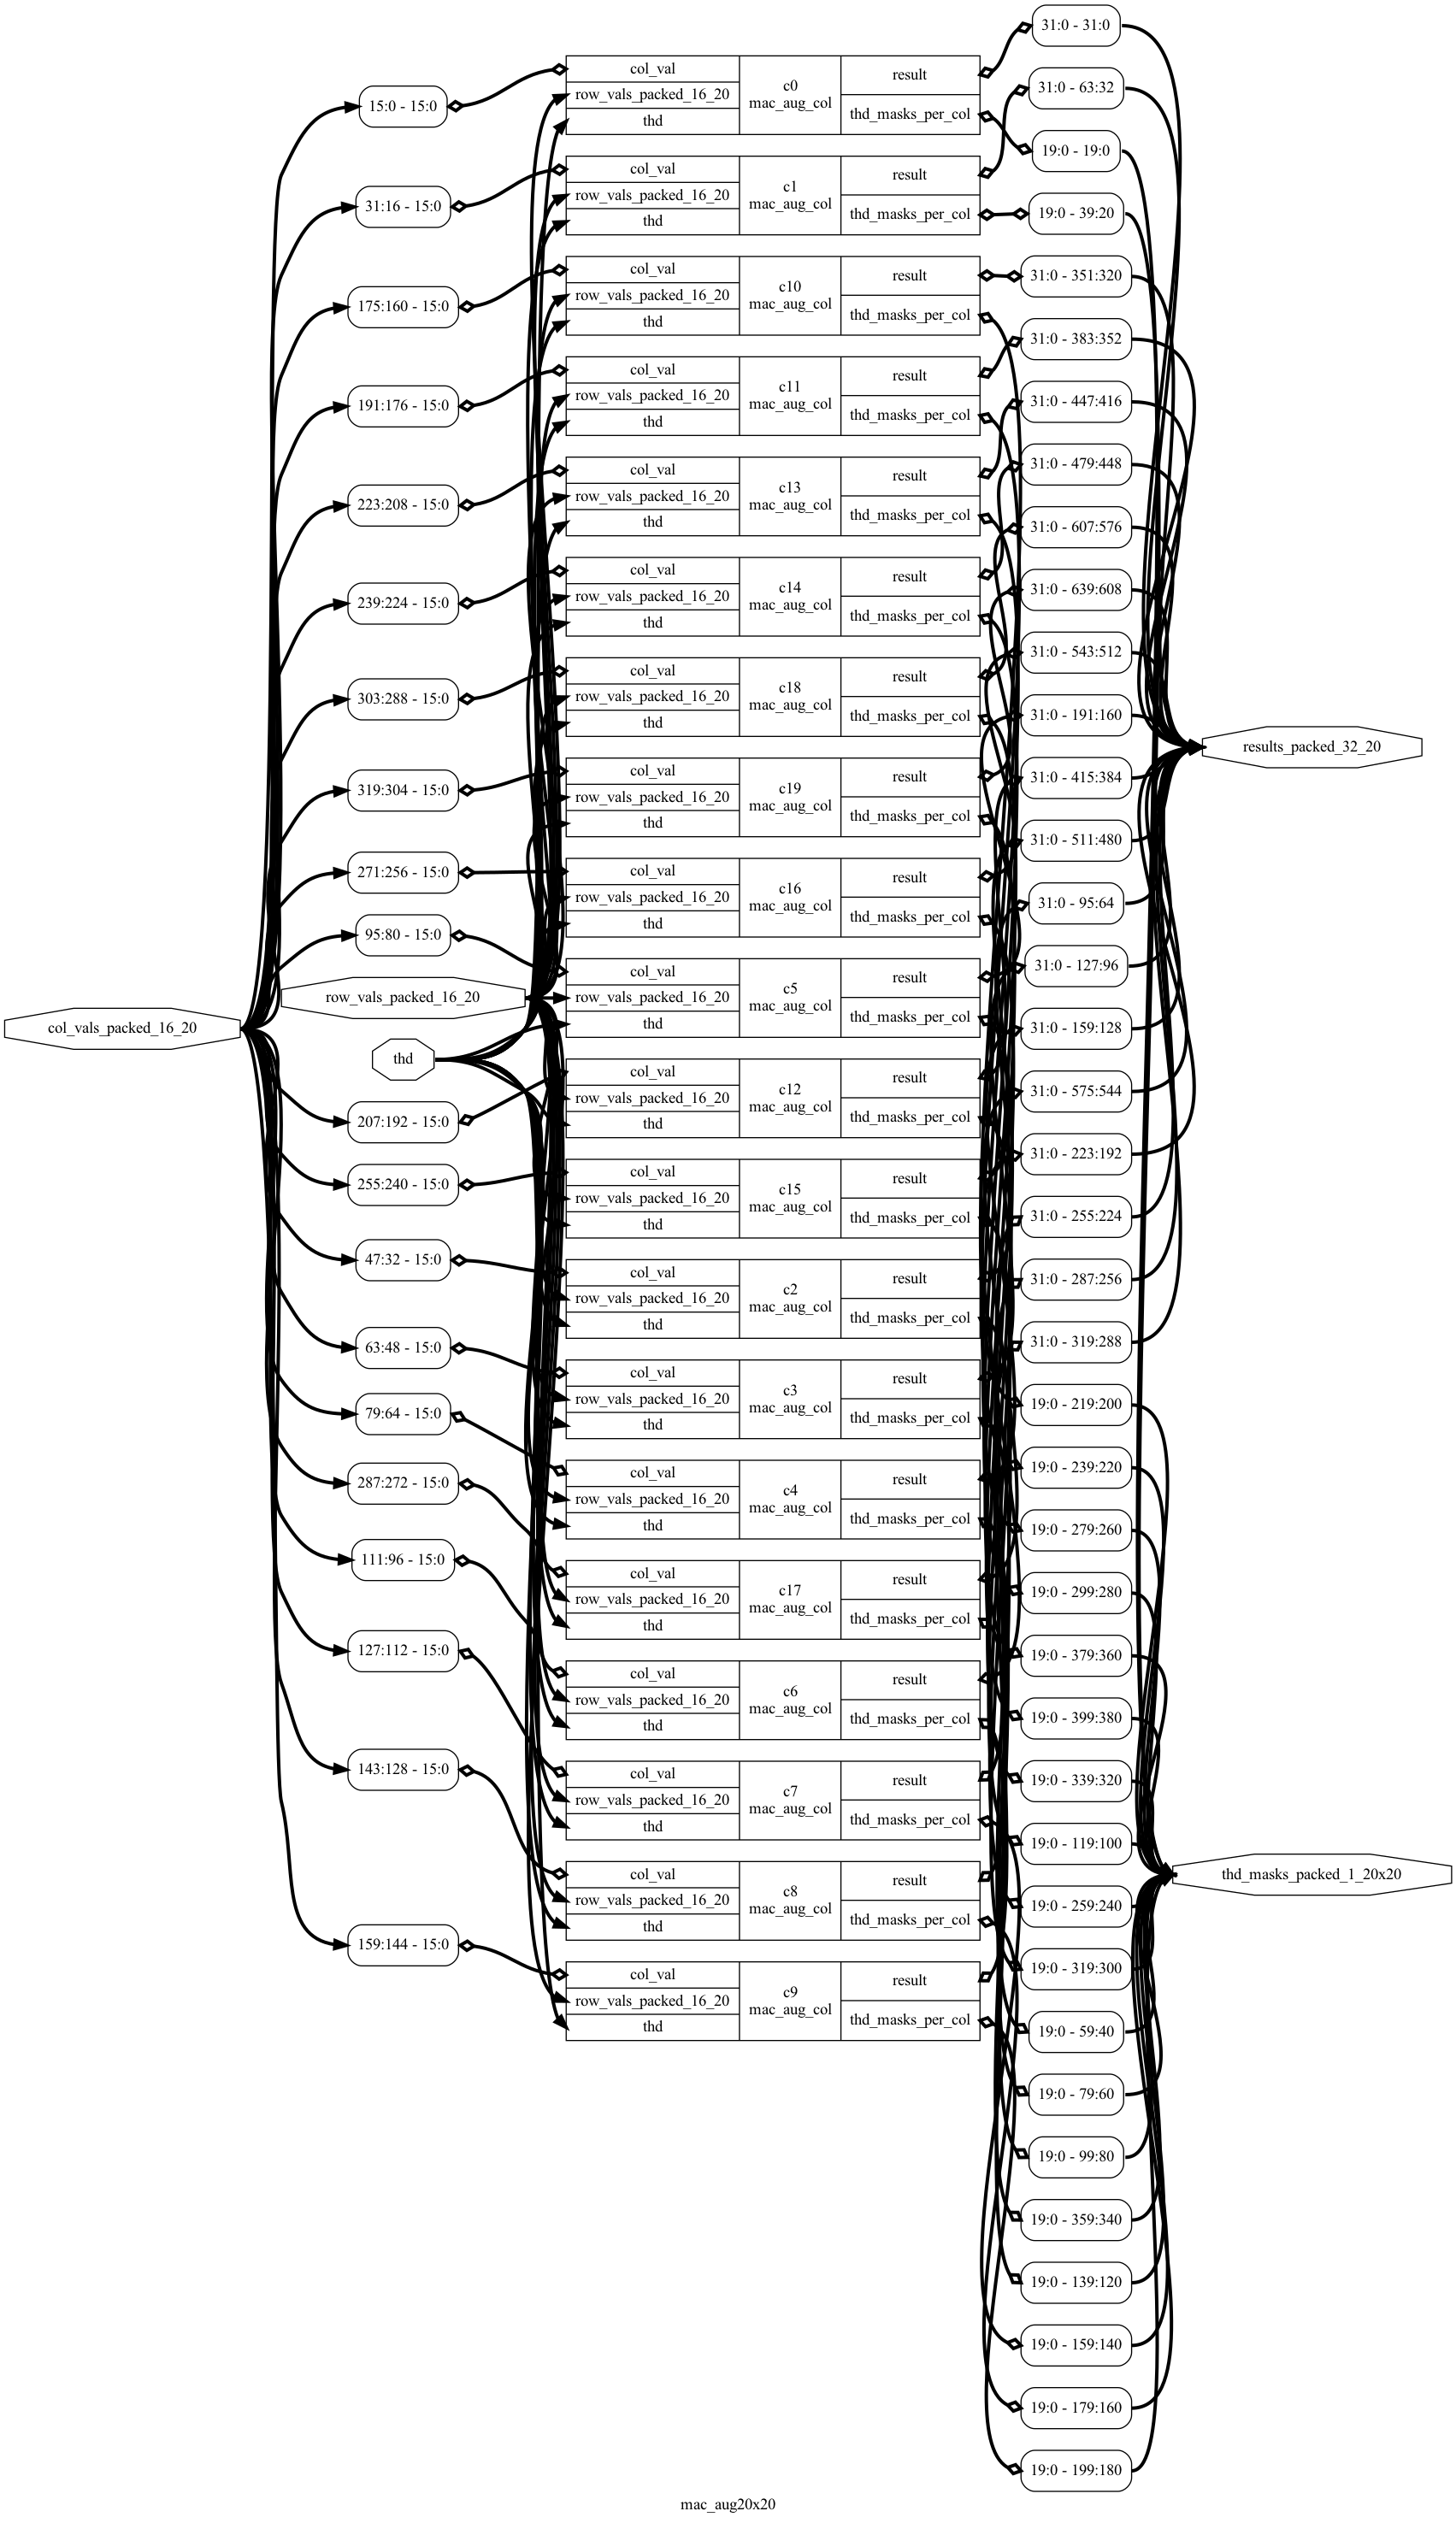
\includegraphics[width=\linewidth]{images/mac_aug20x20.dot.png}
        \caption{20x20 MAC array (augmented)}
      \end{framed}
    \end{subfigure}
    \begin{subfigure}{.45\textwidth}
      \centering
      \begin{framed}
        
\includegraphics[width=\linewidth]{images/mac_aug_col.dot.png}
        \caption{1x20 MAC column (augmented)}
      \end{framed}
      \begin{framed}
        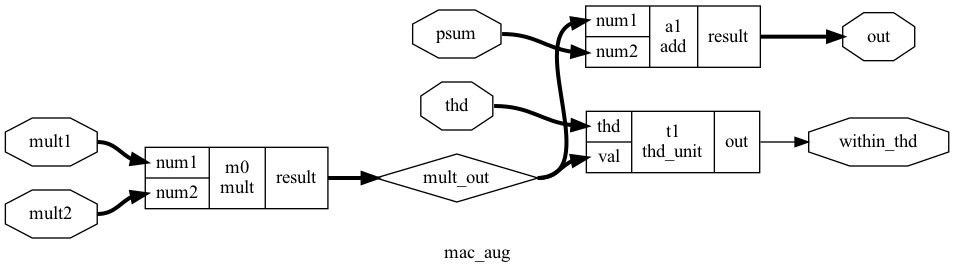
\includegraphics[width=\linewidth]{images/mac_aug.dot.png}
        \caption{Single MAC unit (augmented)}
      \end{framed}
    \end{subfigure}
    \caption{The augmented version of 20x20 MAC array for Ptolemy methods, \underline{BwAb} and \underline{FwAb} is shown. The MAC unit is augmented with a threasholder (\textbf{(c)}), and the 20x20 MAC array is augmented with extra wires to deliver the thresholding results to use as masks in the controller (\textbf{(b), (c)}). The design is syntehsized and visualized with \textbf{yosys}.\label{fig:macs_aug}}
\end{figure}

Figure \ref{fig:mac-aug} show the 20x20 MAC array module with augmentation for \underline{BwAb} and \underline{FwAb} support. Minimal change with a comparator for thresholding is applied to the each MAC unit. Also, additional wires for a threshold input and mask outputs extends original hardware. Test logs for the implementation of augmented 20x20 MAC array module can be found in Appendix \ref{a:mac_aug_test}.

\section{Results}

In this section, we discuss the overhead of Ptolemy's extra hardware requirements. Results are partially complete due to technical problems with using a commercial simulator. However, our estimates present an overall idea of Ptolemy's power/area overhead.

\subsection{Extra SRAM}
\subsubsection{Area Overhead \label{sec:sram-area}}
\begin{table}[H]
    \centering
    \begin{tabular}{cccccc}
    \toprule
    \multirow{2}{*}{\textbf{SRAM}} & \multirow{2}{*}{\textbf{Size}} & \multicolumn{2}{c}{\textbf{Granuality}} & \multicolumn{2}{c}{\textbf{Technology}} \\ \cline{3-6} 
     &  & \textbf{\citet{ptolemy}} & \textbf{Simulated} & \textbf{\citet{ptolemy}} & \textbf{Simulated} \\ \hline
    \textbf{Baseline DNN} & 1.5MB & 64KB & 51KB & 15nm & 22nm \\ \hline
    \textbf{MAC aug.} & 64KB & 2KB & 2KB & 15nm & 22nm \\ 
    \textbf{Path const.} & 32KB & N/A & 2KB & 15nm & 22nm \\ \bottomrule
    \end{tabular}
    \caption{Comparision between configuration used in the Ptolemy paper and in our experiments for SRAM overhead calculation.\label{tab:sram}}
\end{table}

Area overhead is imposed by extra SRAM requirements of Ptolemy. Table \ref{tab:sram} show extra required SRAM. While our simulation configuration is close to original paper's, they are not exactly same due to limitations of \textbf{HP-CACTI}, which we chose as our power/area estimator. We set our estimation configuration to 22nm technology\footnote{Originally, authors used Silvaco's Open 15nm library. Our access request remained unresponsive to the time of writing and we could not use it.} and the granuality to 51KB, which is largest value possible with the chosen estimator.

\begin{table}[H]
    \begin{tabular}{|ccc|ccc|}
    \hline
    \multirow{3}{*}{\textbf{SRAM}} & \multicolumn{2}{c|}{\textbf{Ours (22nm)}} & \multicolumn{3}{c|}{\textbf{\citet{ptolemy} (15nm)}} \\ \cline{2-6} 
     & \multicolumn{2}{c|}{\textbf{SRAM}} & \textbf{SRAM} & \multicolumn{2}{c|}{\textit{\textbf{Overall}}} \\ \cline{2-6} 
     & \textbf{Area($mm^2$)} & \textbf{Overhead (\%)} & \textbf{Area($mm^2$)} & \textit{\textbf{Area($mm^2$)}} & \textit{\textbf{Overhead (\%)}} \\ \hline
    \textbf{Baseline DNN} & 1.786 & - & N/A & \textit{$\approx$1.54} & \textit{-} \\ \hline
    \textbf{MAC aug.} & 0.063 & 2.21 & N/A & \textit{N/A} & \textit{N/A} \\
    \textbf{Path const.} & 0.039 & 3.55 & N/A & \textit{N/A} & \textit{N/A} \\ \hline
    \textbf{MAC + Path} & 0.103 & 5.77 & $\approx$0.06 & \textit{0.08} & \textit{5.2} \\ \hline
    
    \end{tabular}
    \caption{Our measurements of SRAM area compared to reported results in \cite{ptolemy}. Note that some numers are a rough estimate from given available numbers. \label{tab:sram-area}}
\end{table}

Due to different configurations, direct comparison is not possible. Also, \citeauthor{ptolemy} do not provide a breakdown of area overhead. Despite different configurations, we can make some assumptions to compare our experiment results with the \cite{ptolemy}'s result: First, if we assume that ratio of area overhead between SRAM and rest of the hardware is consistent before and after the augmentation, we can say that the percentage overhead incurred by SRAM should have equal percentage value with overall area overhead incurred by augmentation. If this assumption holds true, estimate our SRAM overhead, 5.77\% is very close to the provided augmentation overhead of 5.2\% (Table \ref{tab:sram-area}). Also, we can make a second assumption, that a 22nm synthesized design should be 2.15($\approx(22nm/15nm)^2$) times to that of 15nm synthesized design. If this holds, the measurements of the area of SRAM using 22nm technology should be close to 0.129$mm^2$, which is very close to measurement of 0.103$mm^2$. Under both or either of these assumptions, we dim that our estimates provide some reliability.

Overall, Ptolemy's extra SRAM requirement provide a small footprint of 5.8\% overhead. Also, if assume only \underline{BwAb} and \underline{FwAb} methods, there is no need for the current path constructor. Ideally, we can replace the path constructor with a minimal controller comprised of a series of AND logic gates and a bit accumulator. Thus, with respect to our design choices, Ptolemy's $\mathbf{Overhead_{area}}$ can be in range, $2.21\%<\mathbf{Overhead_{area}}\leq5.77\%$. This is should be a negligible requirement for most design usecases.

\subsubsection{Energy Overhead}

\begin{table}[H]
  \begin{tabular}{ccccccc}
  \toprule
  \multirow{2}{*}{\textbf{SRAM}} & \multicolumn{2}{c}{\textbf{Dynamic read energy}} & \multicolumn{2}{c}{\textbf{Dynamic write energy}} & \multicolumn{2}{c}{\textbf{Standby leakage}} \\ \cline{2-7} 
   & \textbf{nJ} & \textbf{Overhead (\%)} & \textbf{nJ} & \textbf{Overhead (\%)} & \textbf{mW} & \textbf{Overhead (\%)} \\ \hline
  \textbf{Baseline DNN} & 0.150 & - & 0.155 & -- & 447.072 & - \\ \hline
  \textbf{MAC aug.} & 0.022 & 14.82 & 0.033 & 21.42 & 19.696 & 4.41 \\
  \textbf{Path const.} & 0.018 & 12.23 & 0.024 & 15.21 & 10.119 & 2.26 \\ \hline
  \textbf{MAC + Path} & 0.041 & 27.05 & 0.057 & 36.63 & 29.815 & 6.67 \\ \bottomrule
  \end{tabular}
  \caption{Estimate of energy usage for SRAM within each hardware module. \label{tab:sram-energy}}
  \end{table}

  There is no breakdown of energy estimate in \cite{ptolemy} to compare. However, as we use the same software and configurations as used in Section \ref{sec:sram-area}, under same assumption, we dim provided numbers to be reliable to a rough degree.

  Ptolemy hardware impose 27.05\%, 36.63\%, and 29.82\% extra overhead each in dynamic read energy, dynamic write energy, and standby leakage. Again, the minimum threasholder augmentation to the 20x20 MAC array and a minimal controller is enough to power \underline{BwAb} and \underline{FwAb} algorithms of Ptolemy. If such design choice should be made, the extra overhead can be reduced close to 14.82\%, 21.42\%, and 4.41\% in dynamic read energy, dynamic write energy, and standby leakage.
  
\subsection{MAC Augmentation}

\subsubsection{Area Overhead}

\begin{table}[H]
  \centering
  \footnotesize
  \begin{tabular}{|c|cccccc|}
  \hline
  Design & Wires & Public wires & \multicolumn{1}{l|}{Total wires} & Wire bits & Public wire bits & Total wire bits \\ \hline
  MAC 20x20 & 1973643 & 1044443 & \multicolumn{1}{l|}{3018086} & 3718000 & 2065600 & 5783600 \\
  MAC 20x20 (aug.) & 2052885 & 1046485 & \multicolumn{1}{l|}{3099370} & 3995072 & 2106272 & 6101344 \\
  $\Delta$ & 4.02\% & 0.20\% & \multicolumn{1}{l|}{2.69\%} & 7.45\% & 1.97\% & 5.49\% \\ \hline
  Design & AND & MUX & NOT & OR & XOR & Total cells \\ \hline
  MAC 20x20 & 693600 & 108800 & 140800 & 492000 & 326000 & 1761200 \\
  MAC 20x20 (aug.) & 790800 & 108800 & 166400 & 520800 & 366000 & 1952800 \\
  $\Delta$ & 14.01\% & 0.00\% & 18.18\% & 5.85\% & 12.27\% & 10.88\% \\ \hline
  \end{tabular}
  \caption{Area statistics in terms of number of wires and cells.\label{tab:cells}}
\end{table}

As exact specification of area overhead given a number of wires and cells is different for choice of technology, number of wires and cells can be used as a more generic indicator of area overhead. Area overhead from ptolemy augmentation within the main compute unit of DNN accelerator (20x20 MAC array) is provided in Table \ref{tab:cells}. On average, area overhead induced in terms of number of wires, wire bits and cells are 2.69\%, 5.49\%, and 10.88\% each.

\subsubsection{Energy Overhead}

We tried but couldn't utilize commercial simulator software to simulate our design's power usage. As we confirmed synthesis of our verilog code with \textbf{yosys}, we presume that estimating the energy overhead for our synthesized results could have been an easy task. However, due to lack of familiarity in software and ECE server environment and with no access to tutorials, we couldn't get the results in time.

\section{Conclusion}

As \citeauthor{ptolemy} provided, Ptolemy runs on minimally appended hardware and impose small area overhead. However, as we see from our estimation, energy overhead is non-trivial as dynamic read and dynamic write to required extra SRAM module causes 27.05\% and 36.63\% each. We show that further design choice can reduce such overhead. When only adding hardware support for the most efficient variants of Ptolemy, \underline{FwAb} and \underline{BwAb}, the energy overhead for dynamic read and write can reduce to 27.05\%, 36.63\%. Yet, our investigation remain incomplete. We leave our deficiency to future research.

\section{Future Work}

First, we can further study the power overhead of augmented MAC arrays for finer grained design choices for Ptolemy. The original paper suggests \textit{algorithmic knobs} to leverage between accuracy and computation. One of them is deciding which layer to start computing (\underline{FwAb}) or which layer to end computing (\underline{BwAb}) for thresholding methods. However, such approach is too coarse for many neural networks as layers of in a network may vary greatly in number of multiply-add operations. Even AlexNet exhibits extremely varying computation load per layer (See Table \ref{tab:alexnet} in Appendix \ref{a:alex}).

We believe that we can further study the power overheads within finer-grained classes (e.g. filters in a convolutional layer, a subset of neurons in a dense layer) to better understand the power-accuracy trade-off and possibily come up with further optimization techniques.



\bibliography{references}




\newpage
\appendix
\section{Test Logs}

\subsection{20x20 MAC Array \label{a:mac_test}}
Here, test logs are presented. First row show first 3 elements in the input column. Then in each line an element in the input row is shown followed by 3 x's that denote multiply-add. Final row contain 3 first results out of all 20. Note that MAC results correspond to the inputs from previous clock as there exists 1 clock delay (1 clock is 250mHz as in \cite{ptolemy}).

\begin{multicols}{3}
{\tiny \verbatiminput{images/mac20x20_test.txt}}    
\end{multicols}

\subsection{20x20 MAC Array with Augmentation for \underline{BwAb}, \underline{FwAb} Support\label{a:mac_aug_test}}
The test logs are similar to Appendix \ref{a:mac_test}. However, instead of x's now mask bit values are shown. If the absolute value of a psum in the corresponding position is below threshold, 1 is shown. 0, if otherwise. Here exists 1 clock delay as well.


\begin{multicols}{3}
    {\tiny \verbatiminput{images/mac_aug20x20_test.txt}}    
\end{multicols}


\section{Design Implementations and Example Scripts}
Please refer to \url{https://github.tamu.edu/CSCE-614-Dr-Kim-Fall-21/InsooChung}.

\section{AlexNet Multiply-Add Statistics\label{a:alex}}

\begin{table}[H]
  \centering
  \tiny
  \begin{tabular}{ccccccccccc}
  \hline
  \multicolumn{2}{c}{\textbf{Layer}} & \multicolumn{5}{c}{\textbf{Layer Parameters}} & \multicolumn{4}{c}{\textbf{Multiply-Add Operations}} \\ \hline
  \textbf{Name} & \textbf{Type} & \textbf{Dim 1} & \textbf{Dim 2} & \textbf{Depth} & \textbf{Strides} & \textbf{Padding} & \textbf{\#} & \textbf{\%} & \textbf{Bwd Accum \%} & \textbf{Fwd Accum \%} \\ \hline
   & Input & 227 & 227 & 3 &  &  &  &  &  &  \\
  Layer 1 & Conv & 11 & 11 & 96 & 4 &  & 37410054 & 32.55\% & 100.00\% & 32.55\% \\\hline
   & Output & 55 & 55 & 96 &  &  &  &  &  &  \\
   & MaxPool & 3 & 3 &  & 2 &  &  &  &  &  \\
   & Input & 27 & 27 & 96 &  &  &  &  &  &  \\
  Layer 2 & Conv & 5 & 5 & 256 & 1 &  & 4665600 & 4.06\% & 67.45\% & 36.61\% \\\hline
   & Output & 27 & 27 & 256 &  &  &  &  &  &  \\
   & MaxPool & 3 & 3 &  & 2 &  &  &  &  &  \\
   & Input & 13 & 13 & 256 &  &  &  &  &  &  \\
  Layer 3 & Conv & 3 & 3 & 384 & 1 & 1 & 584064 & 0.51\% & 63.39\% & 37.12\% \\\hline
   & Output & 13 & 13 & 384 &  &  &  &  &  &  \\
  Layer 4 & Conv & 3 & 3 & 384 & 1 & 1 & 584064 & 0.51\% & 62.88\% & 37.62\% \\\hline
   & Input & 13 & 13 & 384 &  &  &  &  &  &  \\
  Layer 5 & Conv & 3 & 3 & 256 & 1 & 1 & 389376 & 0.34\% & 62.38\% & 37.96\% \\\hline
   & Output & 13 & 13 & 256 &  &  &  &  &  &  \\
   & MaxPool & 3 & 3 &  & 2 &  &  &  &  &  \\
   & Input & 6 & 6 & 256 &  &  &  &  &  &  \\
   & Flatten & 1 & 9216 &  &  &  &  &  &  &  \\
  Layer 6 & Fully-connected &  & 4096 &  &  &  & 37748736 & 32.84\% & 62.04\% & 70.81\% \\\hline
   & Output/Input & 1 & 4096 &  &  &  &  &  &  &  \\
  Layer 7 & Fully-connected &  & 4096 &  &  &  & 16777216 & 14.60\% & 29.19\% & 85.40\% \\\hline
   & Output/Input & 1 & 4096 &  &  &  &  &  &  &  \\
  Layer 8 & Fully-connected &  & 4096 &  &  &  & 16777216 & 14.60\% & 14.60\% & 100.00\% \\\hline
  Total &  &  &  &  &  &  & 114936326 &  &  &  \\ \hline
  \end{tabular}
  \caption{Multiply-add operation related statistics of AlexNet.\label{tab:alexnet}}
  \end{table}

\end{document}